
\chapter{Computer Vision Libraries}
\label{chap:Library}
The libraries installed in this system are: 
\begin{itemize}
\item The hardware motion libraries that were developed by Pravin as shown in \cite{dhake2007real,dhake2007real1}
\item Computer Vision Libraries. 
\end{itemize}
 
This section overviews the Computer Vision Libraries, and it is divided into two subsections. The first section presents the details of the wireframe libraries, and the last section is about the 3D estimation and visualization libraries.

\section{Wireframe Libraries}
\label{sec:Wireframe}
 Defined below are the different functions, that can be used to generate a wireframe from an image. 
\subsection{Image Acquisition}
This Library function is to acquire an image from the camera. Depending on user's choice, the image can be stored either on \textit{SSD} or on the \textit{Memory}. The function can also be used to peruse a previously stored image on the disk. For both cases, a filename and location choice need to be specified.
\paragraph{Synopsis:}
\begin{lstlisting}
ImageMat *ImageAcquisition(int choice, string filename, string key, I_List &I_object);
\end{lstlisting}
\paragraph{Example:}
To use the function defined above the location choice and the filename needs to be specifieds.
\begin{lstlisting}
main(){ 
	.
	.
	.
	int choice;

	cout<< "Enter choice for data acquisition"<< endl;
	cout <<"choice =1 (Stores into SSD with the    
   	        filename of your choice)"<<endl; 
	cout <<"Choice =2 (Stores into matrix (Image_mat)"<<endl;
	cin >> choice; 
	string filename;
	if(choice==1){
	/* enter filename */
		gets(filename);
	}
	/* define key by the user */
	Iinp= ImageAcquisition(2, s1, s1, I_object);
	.
	.
	.
}
\end{lstlisting}

\subsection{Thresholding}
This function could be used for thresholding the image. This function consists of two parameters \textit{Cthreshold} and \textit{RGBparameter}. Cthreshold is an object of structure \textit{coordinates} having x,y, and z values. RGBparameter is an object of structure \textit{RGB} storing RGB threshold values. Currently only thresholding of RGB is provided but the user can add a threshold for points. Refer to Figure \ref{fig:threshRGB}.
\paragraph{Synopsis:}
\begin{lstlisting}
ImageMat *thresholdRGB(ImageMat* Iparameter, coordinates Cthreshold, RGB RGBthreshold, string key, I_List I_object);
\end{lstlisting}
\paragraph{Example:}
\begin{lstlisting}
main(){ 
.
.
.
Iinp = ImageAcquisition(2, s, s, I_object);
ImageMat *Ithresh = thresholdRGB(Isrc, Cthreshold, RGBthreshold, key, I_object);
.
.
.
}
\end{lstlisting}
\begin{figure} [ht] 
    \centering
    \begin{minipage}[b]{0.45\linewidth}
    \centering
    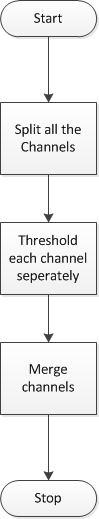
\includegraphics[width=15cm,height=15cm,keepaspectratio]{Pictures/thresholdRGB}
    \caption{Threshold Function}
    \label{fig:threshRGB}
    \end{minipage}
    \begin{minipage}[b]{0.45\linewidth}
    \centering
	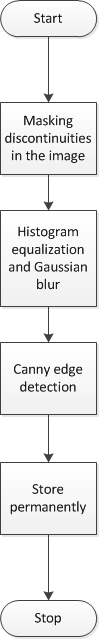
\includegraphics[width=15cm,height=15cm,keepaspectratio]{Pictures/prelimedgedetection}
    \caption{Preliminary Edge Detection}
    \label{fig:prelim}
	\end{minipage}
\end{figure}
\subsection{Preliminary Edge Detection}
 This function detects the edges of the image; The edge detection is preliminary and results in edges that are serrated and not continuous. It is useful in circumstances where the outline of the contents is needed. If a wireframe from the image is desired, preliminary edge detection must be performed. The algorithm is explained in Figure \ref{fig:prelim}.
\paragraph{Synopsis:}
\begin{lstlisting}
ImageMat *PrelimEdgeDetection(ImageMat *Isrc, string key, I_List &I_object);
\end{lstlisting}
\paragraph{Example:}
\begin{lstlisting}
main(){ 
.
.
.
Iinp = ImageAcquisition(2, s, s, I_object);
ImageMat *Iinp=  PrelimEdgeDetection(Iinp, "OriiginalImage", I_object);
.
.
.
}
\end{lstlisting}
\subsection{Vertex Detection}
 This function detects the sure edges of the image, detects the vertices, and combines these vertices to form lines. Prerequisite is that an edge detected image is obtained from prelimedgedetection. The function returns all the points that were detected.
\paragraph{Synopsis:}
\begin{lstlisting}
ImageMat *VerticesDetection(ImageMat *I, string key, P_List &P_ob, L_List &L_ob, I_List &I_ob);
\end{lstlisting}
\paragraph{Example:}
 An example is shown below. The keys that are required to store the points in an associative array needs to be specified. If the keys are not to be permanently be stored then the string '\textit{no}' needs to be sent.
\begin{lstlisting}
main(){ 
.
.
.
ImageMat *Iinp=  PrelimEdgeDetection(Iinp, "OriginalImage", I_object);
Iinp = VerticesDetection(Iinp, "VERTICESIMAGE", P_object, L_object, I_object);
.
.
.
}
\end{lstlisting}
\begin{figure} [ht] 
    \centering
    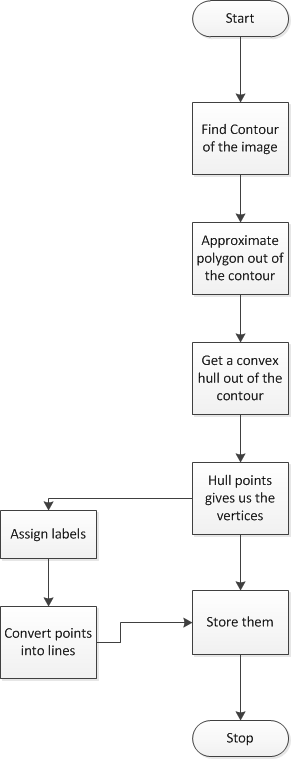
\includegraphics[width=20cm,height=20cm,keepaspectratio]{Pictures/VerticesDetection}
    \caption{Vertices Detection}
    \label{figurespecs1}
\end{figure}

The above functions can be used to generate a wireframe from an image. The process involves finding the edge and the vertices/hull points from an image. These points can be stored at the user's discretion. The user can specifies the value of keys to each of the function to store the data. There are functions provided for the retrieval and removal of keys and the stored data.

The next set of library functions can be used to generate a 3D model from the set of images. A user can use both wireframe and a plain image to create the model. It is advisable that they use the input image to find the various parameters needed to convert the model as it results in increased accuracy but results in decreased speed, hence a tradeoff must be made. While using plain images one needs to convert the image into gray scale.


\section{Visualisation and Motion Libraries}
\label{sec:Wireframe}
The next set of functions would aim at reconstructing a 3D model from a pair of images.
A typical system for the construction of 3D models consists of a stereo rig meaning two-fixed camera, where the relative position of the two cameras are known.
 This operation takes place in three phases. In the
first phase, a set of matched points i.e. pixels in the
two views that are the images of the same point in the
real world are established between the two images.
In the second phase, the identified matched points are
used to derive the relative locations, orientations and
other parameters of the cameras. This process usually
requires iterative solution of a set of non-linear equations. In the third phase the locations of 3D points are
computed. In the current scenario, the modelling is done using a single camera; hence an attempt is made to simulate the stereo vision by moving the camera. This technique is known as structure from motion and is a popular technique in situations where there is no calibrated stereo rig to emulate the left and the right eye. Traditional stereoscopy systems, such as human visual system, utilize multiple viewing angles of the same object in order to do triangulation and get a depth perception, which is the primary objective.


The methodology of Visual Structure
from Motion VSFM is described in \cite{wu2011visualsfm,triggs2000bundle}. The retrieval of 3D model from images is basically divided into a few steps:
\begin{itemize}
\item Point matching and feature extraction,
\item Estimating the camera motion from the pair of images,
\item Point triangulation,
\item Display visualizer.
\end{itemize}

\subsection{Step 1: Feature Extraction and Matching}
The first algorithmic step is \textit{point matching} and \textit{feature extraction}. The main goal here is the matching of one point in one image to the corresponding
point in the other image. During this matching, there are several tasks that the algorithm has to perform.
First, it has to compare the epipolar lines of the images pixel by pixel. For every pixel on one line, the counterpart on the corresponding epipolar line in the other image needs to be identified. After the matching has been done it is possible to calculate how much the pixels have moved in the corresponding images. 

Another method does not involve feature matching. In this method, the optical flow is calculated. The result is the overall flow in the image, but when the motion is large, and the features move substantially in the image, optical flow may fails because pixel movement is usually confined to a search window.  To overcome this problem a hybrid method is implemented in which feature matching is done and these pairs are used as an input flow to calculate the overall motion map. In this method features are extracted first. There are two methods provided by OpenCV library to extract image features. The first method is called \textit{SIFT}, \textit{Scale Invariant Feature Transform} and the second method is \textit{SURF}, \textit{Speeded Up Robust Features}. Even though points can be detected through the vertices detection function mentioned in the previous section, there is a necessity for  recovering the orientation and the details about the neighbors from the image. For this purpose descriptors are neeeded to be detected and recorded from the image. The following section explains the details of the extraction and registration of features. 

The \textit{SIFT} algorithm can be broken down into four main stages: (1) scale-space peak
selection; (2) point localization; (3) orientation assignment; and (4) point descriptor. The first
stage is to search for the points of interest over location and scale. The image is constructed in a
Gaussian Pyramid, where the image is down sampled and blurred at each level. These
blurred images at each level are used to compute the Difference of Gaussians (DoG), that
locates the edges and the corners within an image. Points of Interest are then extracted in stage 2 by
locating the maxima/minima pixels within the different scales of the DoG at the sub-pixel accuracy.
Once points of interest have been located, an orientation is assigned based on the gradient
orientation of the pixels around the point as in \cite{lowe2004distinctive}.

The \textit{SURF Extraction} method approximated the Laplacian of Gaussian with the Difference of Gaussian for finding the invariant features, the same variables are approximated by SURF using the Laplacian of Gaussian with the Box Filter. One big advantage of this approximation is that, the convolution with box filter can be easily calculated with the help of integral images. And it can be performed in parallel for different scales. Also, the SURF algorithm relies on determinant of the Hessian matrix for both scale and location. SURF is a local invariant point of interest detector-descriptor, similar to its predecessor, the accurate but slower SIFT algorithm. In this thesis SURF algorithm is utilized due to its unique rich descriptors and relatively quick processing time. The mathematics and more details refer to \cite{bay2008speeded}.


Both of  these algorithms are robust and accurate for determining the features in an image. In this thesis, these algorithms are used to 
find out the surrounding and neighbors of each special corner in the image. SURF is used for detecting the points, and SIFT is used for defining the descriptors of the same point. \textit{descriptors} belong to an OpenCV provided class to store the surroundings and the orientation of the Gaussian.
Experiments showed that SIFT is slower but more effective in finding descriptors but SURF is more suitable in finding features quickly. Hence the implementation is a combination of both. The points that were detected initially are first filtered by the SIFT algorithm. Some previously detected points may be unsuitable for matching and such points are rejected by the SURF algorithm and the remaining points are used for matching the corresponding points between the two images.

Once features are extracted and their descriptors are calculated, the next step is to match the points and get the relative motion between the points that provides an initial estimation to be used in calculating the overall optical flow. The function, which performs the operations mentioned above, is given below.

\paragraph{Motion Map}
\paragraph{Description}
After points in each frame are detected, disparity between two consecutive images needs to be determined. To determine this disparity two images at two different time instances are provided to the motion map function. This function will calculate optical flow between these images. Optical flow shows where the specific pixels have moved in images, which gives an idea about disparity, which is needed to calculate the third dimension. The user needs to decide which image will be given to the function. The user has the choice of using detected points or standard images. In situations where both the images are actually same the function will give an error message and proceeds forward to the next set of images if the operation is looping as shown in Figure \ref{fig:motionM}.
\paragraph{Synopsis:}
\begin{lstlisting}
int  CalculateMotionMap(Mat img_1, 
						Mat img_2, 
						vector<KeyPoint> &keypoints_1, 
						vector<KeyPoint> &keypoints_2,
						vector<KeyPoint>& fullpts1,
						vector<KeyPoint>& fullpts2,
						vector<KeyPoint> &imgpts1_good,
						vector<KeyPoint> &imgpts2_good,
						vector <DMatch>  &matches);
 \end{lstlisting}
\paragraph{Example:}
 The parameters \textit{img\_1} and \textit{img\_2} are the two images, that are the input to this function. The points, \textit{keypoint\_1} and \textit{keypoint\_2} are the two sets of points that are detected in the image the points.The parameters \textit{imgpts1\_good} and \textit{imgpts2\_good} are the two sets of matched points that are detected in both images. The parameter \textit{fullpts} are all the points which are detected in both the images. The variable Matches provides the corresponding point in the second image for a point in the first image. There are two functions in the library, that convert the library detected points into the keypoints of OpenCV. These functions can be used to convert the user-detected points and send them as parameters to the motion map.
\begin{lstlisting}
main(){  
.
. 
.

ImageMat *Iinp = new ImageMat;
ImageMat *Iinp1 = new ImageMat;

string s = "4.jpg";   
Iinp = ImageAcquisition(2, s, s, I_object);

string s1 = "5.jpg";
Iinp1 = ImageAcquisition(2, s1, s1, I_object);

Iinp=  PrelimEdgeDetection(Iinp, "EdgeImage1", I_object);
\end{lstlisting}
\pagebreak
\begin{lstlisting}
Iinp = VerticesDetection(Iinp, "VERTICESMAGE1", P_object, L_object, I_object);

Iinp1=  PrelimEdgeDetection(Iinp1, "EdgeImage2", I_object);
Iinp1 = VerticesDetection(Iinp1, "VERTICESMAGE2", P_object, L_object, I_object);

/* Wireframe  */

vector<KeyPoint> pt1,pt2;
vector<KeyPoint> imgpts1;
vector<KeyPoint> imgpts2;
vector<KeyPoint> imgpts1_good;
vector<KeyPoint> imgpts2_good;
vector<DMatch>   match;
int sp =  CalculateMotionMap(Iinp->img, 
							 Iinp1->img, 
							 imgpts1, 
							 imgpts2, 
							 pt1, 
							 pt2, 
							 imgpts1_good,
							 imgpts2_good,
							 match);
.
.
\end{lstlisting}
\pagebreak
\begin{lstlisting}
.
}
\end{lstlisting}

\begin{figure} [ht] 
    \centering
    \begin{minipage}[b]{0.45\linewidth}
    \centering
    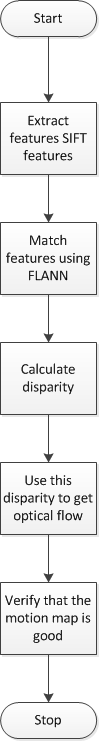
\includegraphics[width=20cm,height=20cm,keepaspectratio]{Pictures/Motionm.png}
    \caption{Motion Map}
    \label{fig:motionM}
    \end{minipage}
    \begin{minipage}[b]{0.45\linewidth}
    \centering
    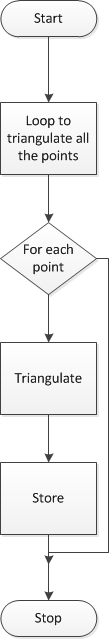
\includegraphics[width=20cm,height=20cm,keepaspectratio]{Pictures/Triangulate}
    \caption{Triangulation}
    \label{fig:Triangulate}
	\end{minipage}
\end{figure}

\subsection{Step 2:  Camera Callibration and Estimation of Camera Matrices}

When working with monocular camera, the spatial relation between the two positions of the camera needs to be known. This relation is given as a rotation and a translation matrix, that provides the transformation between the first and the second positions of the camera. One method to calculate the matrix involves Scalar Vector Decomposition of Essential matrix as described by Hartley and Zisserman in \cite{hartley2003multiple}. 

The primary prerequisite is to know the internal parameters of the camera, which are basically the focal length, and length distortion parameters. They are characterized by matrix $K$ known as the camera callibration matrix and can be calculated using an algorithm proposed by Tsai in \cite{horn2000tsai}. Using this algorithm, the process of calculating the camera calibration matrix can be automated by providing the camera with images of different orientations of a chessboard pattern. The resulting matrix is known as the camera projection matrix. This matrix provides the conversion between, the world coordinate and the camera coordinate frames. 

A simple contrast-based algorithm can recognize the black-white intersections in the chessboard squares. The application of the algorithm generates the camera's internal matrix. There is a camera calibration function provided in the library that makes use of the chessboard pattern to detect all the internal parameters of the camera.

To calculate the unknown dimension of a point in the image, a tansformation called Fundamental Matrix needs to be determined. It is the algebraic representation of epipolar geometry as explained in \cite{hartley2003multiple}. To elaborate, the epipolar geometry is the intrinsic projective geometry between two view or images of the same scene. It is independent of scene structure, and it only depends on the camera's internal parameters and relative position and orientation. The fundamental matrix F encapsulates this intrinsic geometry. It is a matrix of size \(3{\times}3\) and rank 2. 
\begin{figure} [htb!] 
    \centering
    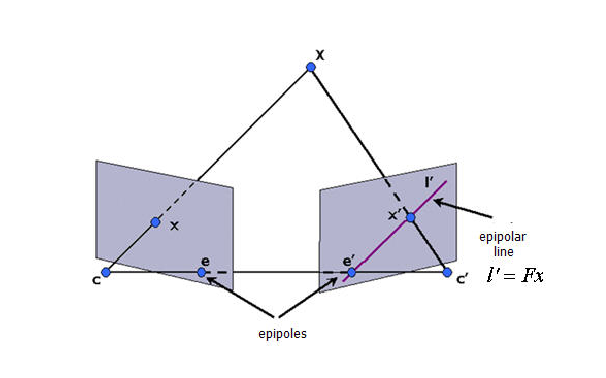
\includegraphics[width=15cm,height=15cm,keepaspectratio]{Pictures/epipolar.png}
    \caption{Epipolar Geometry}
    \label{figure:epi}
\end{figure}
 Defined below are some definitions as given in Hartley and Zissermann \cite{hartley2003multiple}, that elaborate more on the details of the epipolar geometry.
\begin{itemize}
\item  An epipole is the point of intersection of the line joining the camera centers also known as baseline, with the image plane. 
\item  The epipolar plane is a plane containing the baseline. 
\item  An epipolar line is the intersection of an epipolar plane with the image plane.
All epipolar lines intersect at the epipole. An epipolar plane intersects the two image planes in epipolar lines,
 and defines the correspondence between the lines.
\end{itemize}


A particular point captured by a camera has a two dimensional representation in the camera coordinate system described by 
	\[
  x=
  \left[ {\begin{array}{c}
    x1 \\
   x2  \\
	1 \\
  \end{array} } \right]
\] 
The same point described in a different image would have different values described by 
\[
  x'=
  \left[ {\begin{array}{c}
    x1' \\
   x2'  \\
	1 \\
  \end{array} } \right]
\] 
The fundamental matrix relates the two points in such a way that \(x^{T}Fx'=0 \) as described in \cite{hartley2003multiple}.
In \cite{torr1997development,hartley2003multiple} the methods to derive the Fundamental matrix are explained.
In Figure \ref{figure:epi}, $C$ represent the camera centers. The point $X$ is the point in the environment which is pictured by camera in two views as $x$ and $x'$. The line joining the two camera centers is the baseline and the plane containing the points $X$, $x$ and $x'$ is denoted by $\pi$. 

  It is shown in Figure \ref{figure:epi} that the points $x$, $x'$ and $X$ are coplanar and lie in plane $\pi$. It can also  be seen in the figure that the rays from the camera centers of both the images intersect at $X$ and the rays are also coplanar.


Hence given a pair of images, it can established that for each point $x$  in one image, there exists a corresponding line l' in the second image of the same scene, that is the line connecting camera center and the world point. A point in the second image corresponding to the point in the first image must lie on the epipolar line as the epipolar line is the projection in the second image of the ray joining point $x$ and the camera center $C$ of the first image. Thus, there exists a mapping from a point in one image to its corresponding epipolar line in the other image. F, the fundamental matrix encapsulates this information
OpenCV provides functions to iteratively find the Fundamental Matrix as explained in \cite{hartley2003multiple}. 


For a callibrated camera, a normalized coordinate system provides more accurate mapping information, In this case, a specialisation of the Fundamental matrix known as Essential matrix is utilized. This matrix can be expressed as  \[ E = {K'}^T F K\] where F is the Fundamental matrix and K is the camera callibration matrix.

Once the essential matrix is known, the camera matrices defining the transformation may be retrieved from E. In contrast with the fundamental matrix case, where there is a projective ambiguity during reconstruction, the camera matrices may be retrieved from the essential matrix up to
scale and a four-fold ambiguity, meaning there are four possible solutions, except for
overall scale, which cannot be determined.  

The projection matrix $P$, that can be derived from the essential matrix is the transformation between the relative positions of the camera but include the effect of the camera callibration matrix. It is given as the product of \( P = K [R  |  t] \)
where  \([R  |  t] \) is given by 

	\[\left[ \begin{array}{ccc}
   \cos \theta & \sin \theta & Tx\\
   -\sin \theta & \cos \theta & Ty \\
   0 & 0 & 1 \\
  \end{array} \right]\] 
So if the calibration matrix K is known, then the matrix \(K^{-1} P\) is 
called the normalized camera matrix, the effect of the known calibration matrix having
been removed. The resulting projection matrix is the the transformation between the cameras with normalized coordinates and is used to predict the position of the camera. For this purpose the normalized matrix is saved at each motion sequence to track the object motion from the initial reference point which is assumed to be identity. 

 The function described below is provided in the library to calculates the required camera matrices.

\paragraph{Find Camera Matrices}
\paragraph{Description}
This functions calculates both the essential matrix and the Fundamental matrix.
\pagebreak
\paragraph{Synopsis:}
\begin{lstlisting}

bool FindCameraMatrices(const Mat& K, 
						const Mat& Kinv, 
						const Mat& distcoeff, 
						const vector<KeyPoint>& imgpts1, 
						const vector<KeyPoint>& imgpts2, 
						vector<KeyPoint>& imgpts1_good, 
						vector<KeyPoint>& imgpts2_good, 
						Matx34d& P, Matx34d& P1, 
						vector<DMatch>& matches, 
						vector<CloudPoint> &outCloud); 

 \end{lstlisting}
\paragraph{Example:}
The variables $K$ and $Kinv$ are the camera internal parameters as provided by the callibration of the camera.
\begin{lstlisting}
main(){
.
.
.
v::Mat K, Kinv ;
cv::Mat cam_matrix, distortion_coeff;
std::vector<CloudPoint> pointcloud;
std::vector<cv::KeyPoint> correspImg1Pt;
\end{lstlisting}
\pagebreak
\begin{lstlisting}
cv::FileStorage fs;

fs.open("out_camera_data.xml",cv::FileStorage::READ);
fs["Camera_Matrix"]>>cam_matrix;
fs["Distortion_Coefficients"]>>distortion_coeff;
K = cam_matrix;
invert(K, Kinv); //get inverse of camera matrix
cout << Kinv<<endl;
int a;
cout<< "cam matrixes"<< K<< endl;

vector<KeyPoint> pt1,pt2;
vector<KeyPoint> imgpts1;
vector<KeyPoint> imgpts2;
vector<KeyPoint> imgpts1_good;
vector<KeyPoint> imgpts2_good;
vector<DMatch>   match ;

Matx34d    P = cv::Matx34d(1,0,0,0,
                        0,1,0,0,
                        0,0,1,0);
Matx34d    P1 = cv::Matx34d(1,0,0,50,
                         0,1,0,0,
                         0,0,1,0);
\end{lstlisting}
\pagebreak
\begin{lstlisting}
int sp =  CalculateMotionMap(Iinp->img, 
							 Iinp1->img, 
							 imgpts1, 
							 imgpts2, 
							 pt1, 
							 pt2, 
							 imgpts1_good,
							 imgpts2_good,
							 match);

bool s = FindCameraMatrices( K, 
						Kinv, 
						distcoeff, 
						imgpts1, 
						imgpts2, 
						imgpts1_good, 
						imgpts2_good, 
						P, 
						P1, 
						matches, 
						&outCloud); 
.
.
.
}
\end{lstlisting}

\pagebreak
\begin{figure} [ht] 
    \centering
    \begin{minipage}[b]{0.45\linewidth}
    \centering
    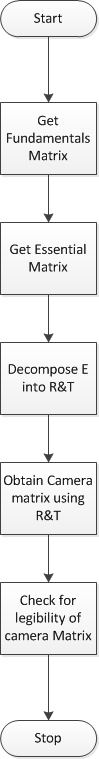
\includegraphics[width=20cm,height=20cm,keepaspectratio]{Pictures/FCM.png}
    \caption{Finding Camera Matrices}
    \label{fig:motionM}
    \end{minipage}
\end{figure}
\pagebreak
 \begin{figure}[ht]
    \centering
    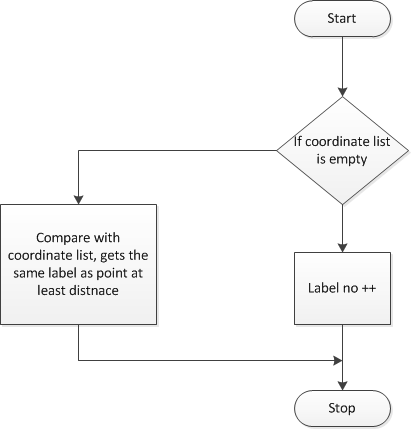
\includegraphics[width=15cm,height=15cm,keepaspectratio]{Pictures/AL}
    \caption{Assigning Labels}
    \label{fig:Triangulate}
	\end{figure}
\pagebreak



\subsection{Step 3: Triangulation and  Image Reconstruction}
After the camera matrices are calculated, the next step in the process is to calculate the unknown dimension of the image, this calculation is done by triangulation of the corresponding points and the camera location. The linear triangulation method is the most common one, described, for instance, in~\cite{hartley2003multiple}. 

The method involves calculating the unknown dimension by searching for the best possible solution which satisfies the fundamental matrix relation of the corresponding points. This search is reduced by knowledge of the epipolar geometry of corresponding points. The point in the 3D space must lie on the intersection of the line passing through the camera center and the point on the image plane for both the images. The result of this search is the identified 3D space coordinate points.

% If a point in the world coordinate is represented as $x$, then the projection on the camera plane is given by
% \(u = Px\). In homogeneous coordinates, \(u = w(u, v, 1)^{T}\) where \(u\) and \(v\) are the observed point coordinates, and $w$ is the unknown scale factor of the coordinate system. 
% In the equation $u = Px$, if the rows of the matrix $P$ is represented by $p_i$, then
% \[wu ={p_1}^Tx, wv ={p_2}^Tx, w={p_3}^T\]

% Eliminating w using the third equation, 
% \[up_3^T x = p_1^T‬x\]
% \[vp_3^Tx =p_x^T.\]

% Four linear equations are obtained in the coordinates of x, which may be written in the form
% \(Ax=0\) for a suitable \(4 {\times}4\) matrix, A. Solving these equation the third dimension of a point may be found.
% These equations define x only up to an in determinant scale factor, and a nonzero solution for x is obtained.

The end solution on triangulation is the third dimension of a point corrected upto a scale factor. 
The scale factor error can be removed but it needs a set of ground control points. 
This would require extra hardware and is not feasible as part of this project.
At the end of this step points with a third dimension detected and stored in a point cloud. It is a collection of the points, computed in the earlier steps, displayed in an OpenGL implemented viewer.
\pagebreak
\paragraph{Triangulate Points}
\paragraph{Description}
 This function calcualtes the 3rd dimension and it is stored as part of the point structure defined in this system. Figure \ref{fig:Triangulate}
\paragraph{Synopsis:}
\begin{lstlisting}
double TriangulatePoints(const vector<KeyPoint>& pt_set1, 
                         const vector<KeyPoint>& pt_set2, 
                         const Mat& K,
                         const Mat& Kinv,
                         const Mat& distcoeff,
                         const Matx34d& P,
                         const Matx34d& P1,
                         vector<CloudPoint>& pointcloud,
                         vector<KeyPoint>& correspImg1Pt);
 \end{lstlisting}

 In this function, \textit{pt\_set1} and \textit{pt\_set2} are all the points detected in the images. \textit{K} and \textit{Kinv} are the camera callibration matrices . The variable pointcloud is a vector array in accordance with the point cloud library that is used in this system to visualize the 3D model. This function is called from inside the FindCameraMatrices function which gives the point cloud as output, but if the user needs to call this function from main,  it could be  done after calling FindCameraMatrices function. 

\section{functions for Display, storage and other primary low level functions}
\paragraph{Convert to Grayscale}
\paragraph{Description}
Image input in OpenCV is generally three-channel image (RGB) and this function can be used to convert into grayscale.
\paragraph{Synopsis:}
\begin{lstlisting}
ImageMat *imageconvertgrayscale(ImageMat *I);
\end{lstlisting}


\paragraph{ Retrieve Image from Storage}
\paragraph{Description}
This function retreives image from the permanent storage using the time key and the string key. 
\paragraph{Synopsis:}
\begin{lstlisting}
ImageMat retreiveimages(I_List &I, time_t t, string key);
\end{lstlisting}

\paragraph{ Retrieve Lines from Storage}
\paragraph{Description}
This function  retreives lines from the permanent storage using the time key and the string key. 
\paragraph{Synopsis:}
\begin{lstlisting}
lines *retreivelines(L_List &L, time_t t, string key);
\end{lstlisting}


\paragraph{ Retrieve Points from Storage}
\paragraph{Description}
This function  retreives points from the permanent storage using the time key and the string key. 
\paragraph{Synopsis:}
\begin{lstlisting}
point retreivepoints(P_List &P, time_t t, string key);
\end{lstlisting}

\paragraph{ Retrieve Camera Motion from  Storage}
\paragraph{Description}
This function retreives image from the permanent storage using the time key.  
\paragraph{Synopsis:}
\begin{lstlisting}
void retreivemotion(M_List &M, time_t t);
\end{lstlisting}


\paragraph{ Erase Lines from Storage}
\paragraph{Description}
This function can be used to erase lines from the permanent storage.
\paragraph{Synopsis:}
\begin{lstlisting}
void eraselines(L_List &L, time_t t, string key);
\end{lstlisting}


\paragraph{ Erase Points from Storage}
\paragraph{Description}
This function can be used to erase points from the permanent storage.
\paragraph{Synopsis:}
\begin{lstlisting}
void erasepoints(P_List &P, time_t t, string key);
\end{lstlisting}

\paragraph{ Erase Images from Storage}
\paragraph{Description}
This function can be used to erase images from the permanent storage. 
\paragraph{Synopsis:}
\begin{lstlisting}
void eraseimages(I_List &I, time_t t, string key);
\end{lstlisting}


\paragraph{ Erase Camera Motion from  Storage}
\paragraph{Description}
This function can be used to erase camera motion from the permanent storage.
\paragraph{Synopsis:}
\begin{lstlisting}
void erasemotion(M_List &M, time_t t );
\end{lstlisting}


\paragraph{ Store  Images into  Storage}
\paragraph{Description}
This function can be used to store images into the permanent storage. 
\paragraph{Synopsis:}
\begin{lstlisting}
void storeimage(I_List &I, ImageMat M, string key);
\end{lstlisting}

\paragraph{ Store  Points into  Storage}
\paragraph{Description}
This function can be used to store points into the permanent storage. 
\paragraph{Synopsis:}
\begin{lstlisting}
void  storepoints(P_List &P, point *p, string key);
\end{lstlisting}

\paragraph{ Store  Lines into  Storage}
\paragraph{Description}
This function can be used to store lines into the permanent storage. 
\paragraph{Synopsis:}
\begin{lstlisting}
void  storelines(L_List &L, lines l, string key);
\end{lstlisting}


\paragraph{ Store  Motion into  Storage}
\paragraph{Description}
This function can be used to store motion into the permanent storage. 
\paragraph{Synopsis:}
\begin{lstlisting}
void storemotion(M_List &M, Matx34d P);
\end{lstlisting}


\paragraph{Remove the keys}
\paragraph{Description}
Two overloaded functions are provided to remove the keys from the storage of keys.
\paragraph{Synopsis:}
\begin{lstlisting}
void remove(vector<time_t> &v, time_t & item);
void remove(vector<string> &v, string & item);
\end{lstlisting}


\paragraph{Display all the keys}
\paragraph{Description}
This function displays all the string keys. 

\paragraph{Synopsis:}
\begin{lstlisting}
void Display_All_Keys_string(list<string> L);
\end{lstlisting}



\paragraph{Display all the keys}
\paragraph{Description}
This function displays all the time keys. 
\paragraph{Synopsis:}
\begin{lstlisting}
void Display_All_Keys_time(list<time_t> L);
\end{lstlisting}


\paragraph{Compare Points}
\paragraph{Description}
This function can be used to compare two points to know if they are equal in the line. 
\paragraph{Synopsis:}
\begin{lstlisting}
int comparepoints(lines *temp, lines *temp1);
\end{lstlisting}


\paragraph{Convert  Points into lines }
\paragraph{Description}
This function can be used to convert detected points into lines.
\paragraph{Synopsis:}
\begin{lstlisting}
lines *convert(point *V);
\end{lstlisting}



\paragraph{Display Points on an Image }
\paragraph{Description}
 This function can be used to display all the detected points on an image.
\paragraph{Synopsis:}
\begin{lstlisting}
Mat Display_Points_onImage(point *Vertexes, Mat im_bw1);
\end{lstlisting}


\paragraph{Assign labels to all the points}
\paragraph{Description}
This function can be used for assigning labels to all the points useful for tracking purposes. 
\paragraph{Synopsis:}
\begin{lstlisting}
point *assignlabels(point *V);
\end{lstlisting}




\paragraph{Matches to Points}
\paragraph{Description}
 This function can be used to convert from OpenCV matches into keypoints defined by the library. 
\paragraph{Synopsis:}
\begin{lstlisting}

void matches2points(const vector<KeyPoint>& train, 
         			const vector<KeyPoint>& query,
           			const std::vector<cv::DMatch>& mtches, 
           			std::vector<cv::Point2f>& pts_train,
           			std::vector<Point2f>& pts_query);

\end{lstlisting}
\paragraph{Keypoints to Points}
\paragraph{Description}
This function converts the feature points in an image to points in 2d, which can be stored into the custom defined data structures provided by the library.
\paragraph{Synopsis:}
\begin{lstlisting}
void PointsToKeypoints(const vector<Point2f>& in, 
			             vector<KeyPoint>& out);
\end{lstlisting}


\paragraph{Points to keyPoints}
\paragraph{Description}
 This is an OpenCV required conversion for reconstruction. It converts the points in 2d into feature points in an image. 
\paragraph{Synopsis:}
\begin{lstlisting}
void PointsToKeypoints(const vector<Point2f>& in, 
						vector<KeyPoint>& out);
\end{lstlisting}




\paragraph{Points to keyPoints}
\paragraph{Description}
 This function can be used to align all matched points in both the images for triangulation using the matches. 
\paragraph{Synopsis:}
\begin{lstlisting}
void GetAlignedPointsFromMatch(const vector<cv::KeyPoint>& imgpts1,
                                const vector<cv::KeyPoint>& imgpts2,
                                const vector<cv::DMatch>& matches,
                                vector<cv::KeyPoint>& pt_set1,
                                vector<cv::KeyPoint>& pt_set2);
\end{lstlisting}





\paragraph{Scalar Vector Decomposition}
\paragraph{Description}
 This function is used to take scalar vector decomposition of essential matrix.
\paragraph{Synopsis:}
\begin{lstlisting}
void TakeSVDOfE(Mat_<double>& E, Mat& svd_u, Mat& svd_vt, Mat& svd_w);
\end{lstlisting}




\paragraph{ Decompose Essential Matrix }
\paragraph{Description}
This function is used to decompose E into rotational and the translation matrix.
\paragraph{Synopsis:}
\begin{lstlisting}
bool DecomposeEtoRandT(Mat_<double>& E, Mat_<double>& R1,
                       Mat_<double>& R2, Mat_<double>& t1,
                       Mat_<double>& t2);
\end{lstlisting}

\paragraph{ Check Coherent Rotation }
\paragraph{Description}
 This function can be used to check the credibility of rotation matrix 
\paragraph{Synopsis:}
\begin{lstlisting}
bool CheckCoherentRotation(cv::Mat_<double>& R);
\end{lstlisting}
\paragraph{Get Fundamental Mat}
\paragraph{Description}
This function calculates the fundamental matrix. Refer \cite{hartley2003multiple, hartley1995linear}. 
\paragraph{Synopsis:}
\begin{lstlisting}
Mat GetFundamentalMat(const vector<KeyPoint>& imgpts1, 
					  const vector<KeyPoint>& imgpts2, 
					  vector<KeyPoint>& imgpts1_good, 
					  vector<KeyPoint>& imgpts2_good, 
					  vector<DMatch>& matches);
\end{lstlisting}

\paragraph{ Test Triangulation }
\paragraph{Description}
This function tests the Essential matrix to see which of the four solutions found is the correct one, For this one calculates the third dimension and records the one for which z is positive to determine the best and valid solution.
\paragraph{Synopsis:}
\begin{lstlisting}
bool TestTriangulation(const vector<CloudPoint>& pcloud, 
					   const Matx34d& P, 
					   vector<uchar>& status);
\end{lstlisting}


\paragraph{ Recover Point }
\paragraph{Description}
 This function can be used to get library defined point structure from PCL specialized point cloud 
\paragraph{Synopsis:}
\begin{lstlisting}
point *Recoverpoint(vector<CloudPoint>& pointcloud, point *P);
\end{lstlisting}

\paragraph{ Convert into Point Cloud }
\paragraph{Description}
This function can be used to convert a point structure point into a point cloud, which can be visualized.
\paragraph{Synopsis:}
\begin{lstlisting}
pcl::PointCloud<pcl::PointXYZ>::Ptr convertintopointcloud(point *p, 
				pcl::PointCloud<pcl::PointXYZ>::Ptr cloud,
				int size);
\end{lstlisting}


\paragraph{ Iterative Triangulation }
\paragraph{Description}
This function can be used to do an iterative triangulation to find the third dimension of a point. At least 10 iterations are recommended. Refer \cite{hartley2003multiple, hartley1995linear}. 

\paragraph{Synopsis:}
\begin{lstlisting}
Mat_<double> IterativeLinearLSTriangulation(Point3d u,  
                                            Matx34d P,          
                                            Point3d u1,        
                                            Matx34d P1);
\end{lstlisting}


\paragraph{  To display the 3D point cloud }
\paragraph{Description}
This function can be used to obtain visualization of point cloud.
\paragraph{Synopsis:}
\begin{lstlisting}
void visualization(pcl::PointCloud<pcl::PointXYZ>::Ptr source_cloud);
\end{lstlisting}


\paragraph{ Viewer Generator}
\paragraph{Description}
This function can be used to generate a viewer for the Point Cloud
\paragraph{Synopsis:}
\begin{lstlisting}
boost::shared_ptr<pcl::visualization::PCLVisualizer> simpleVis(pcl::PointCloud<pcl::PointXYZ>::Ptr cloud);
\end{lstlisting}


\paragraph{  To create a mesh from the 3D point cloud }
\paragraph{Description}
 This function can be used to create a mesh from the point cloud, basically triangulates the points into mesh.
\paragraph{Synopsis:}
\begin{lstlisting}
pcl::PolygonMesh pointcloudmesh(pcl::PointCloud<pcl::PointXYZ>::Ptr cloud);
\end{lstlisting}

\section{Other Functions}
This section includes functions, which are necessary for the purpose of the completion of the project and initialization of the various hardware
in the system. This includes the camera calibration function that is not required to be done every time one starts running the code but will be necessary if one changes the camera which will lead to change in the internal parameters of the camera. The functions follows the algorithm given by Tsai in \cite{horn2000tsai}. OpenCV also provides us with various functions, which are helpful in doing the camera calibration, The camera calibration is done using a chess board pattern. The function returns the camera calibration matrix and the distortion parameters.
\paragraph{Synopsis:}
\begin{lstlisting}
Mat cameracalibration(Mat &distortion);
\end{lstlisting}
Another function, is for reading images from the camera through the frame grabber board. This function consists of a modified source code of the sample application given by Sensoray. The function is called from image acquisition and involves activating the frame grabber and reading the image writing it on the hard drive and returning the file name  and loading  it onto the image matrix. 
\paragraph{Synopsis:}
\begin{lstlisting}
void ImagetoSSD(string filename);
\end{lstlisting}





